
%%%%%%%%%%%%%%%%%%%%%%%%%%%%%%%%%%%%%%%%%%
%%%%%%%%%%%%%%%%%%%%%%%%%%%%%%%%%%%%%%%%%%
\section{D$\emptyset$ experiment}

%%%%%%%%%%%%%%%%%%%%%%%%%%%%%%%%%%%%%%%%%%
\subsection{Overview}
%%%%%% SLIDE
\begin{frame}{\textcolor{Goldenrod}{D$\emptyset$ Experiment}}
  \begin{overlayarea}{\textwidth}{\textheight}
    \begin{figure}[h]\centering
      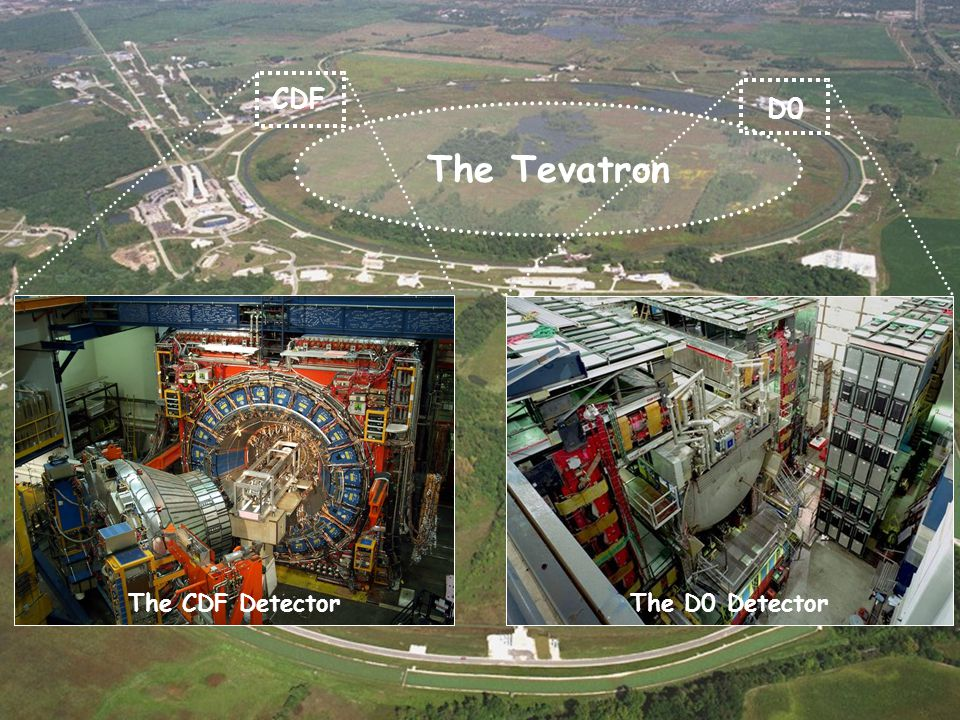
\includegraphics[height=0.5\textheight]{./Images/02_D0_general.jpg}
      \caption*{Aerial view of Fermilab National Accelerator Laboratory}
    \end{figure}
    \itt
  \item[$\Box$] probed $\sqrt{s} = 1.96 TeV$ $p-\bar{p}$ collisions at
    a rate of \alert{$1.2\times 10^{6} s^{-1}$} (\alert{$\approx
      \mathcal{L}_{int} = 10 fb^{-1}$})
    \tti
  \end{overlayarea}
\end{frame}

%%%%%%%%%%%%%%%%%%%%%%%%%%%%%%%%%%%%%%%%%%
\subsection{Experiment goals}
%%%%%% SLIDE
\begin{frame}{\textcolor{Goldenrod}{D$\emptyset$ Experiment Goals}}
  \itt
\item[$\Box$] \hlt{black}{Precision searches:}
\itt
\item Z and W masses, widths and production cross sections
\item Forward-backward asymmetry
\item $W/Z \to q\bar{q}$
\item $\frac{\alpha_{QCD}}{\alpha_{QED}}$ 
\item Gauge boson couplings
  \tti

\item[$\Box$] \hlt{Orange}{New physics:}\\
  \itt
\item $Z \to X \gamma; X\to l^+l^-$
\item top
\item \hlt{Magenta}{Higgs boson   }
\item \hlt{Red}{Supersymmetry}
\item $W', Z'$, heavy leptons and heavy quarks
\item Surprises !
  \tti
  \tti
\end{frame}  

%%%%%%%%%%%%%%%%%%%%%%%%%%%%%%%%%%%%%%%%%%
\subsection{Design considerations}
%%%%%%%% SLIDE
\begin{frame}{\textcolor{Goldenrod}{D$\emptyset$ Design Considerations}}
  \itt
\item[$\bullet$]\textcolor{blue}{Electromagnetic energy resolution at
    the level of $\delta E / E = \frac{0.05}{\sqrt{E}}$ with good
    $\pi^0-\gamma$ separation}
\item[$\bullet$] \textcolor{blue}{good muon momentum resolution and
    muon ID}
\item[$\bullet$] \textcolor{Blue}{Hadron energy resolution of about
    $\delta E / E = \frac{0.8}{\sqrt{E}}$:} {\small
    \itt
  \item \textcolor{Magenta}{$p^{jet}_T, m^{jet}$, and
      $\slashed{E_{T}}$ are critically dependent upon it.} \tti }
\item[$\bullet$] \textcolor{Blue}{Missing transverse energy
    resolution:} {\small
    \itt
  \item \textcolor{Magenta}{angular coverage down to about
      $1^{\circ}$}
  \item minimizing dead areas in the large angle calorimetry
    \tti }
  \tti   
\end{frame}

%%%%%% The upgraded D0
\begin{frame}{\textcolor{Goldenrod}{Upgraded D$\emptyset$}}
  \begin{figure}[h]
    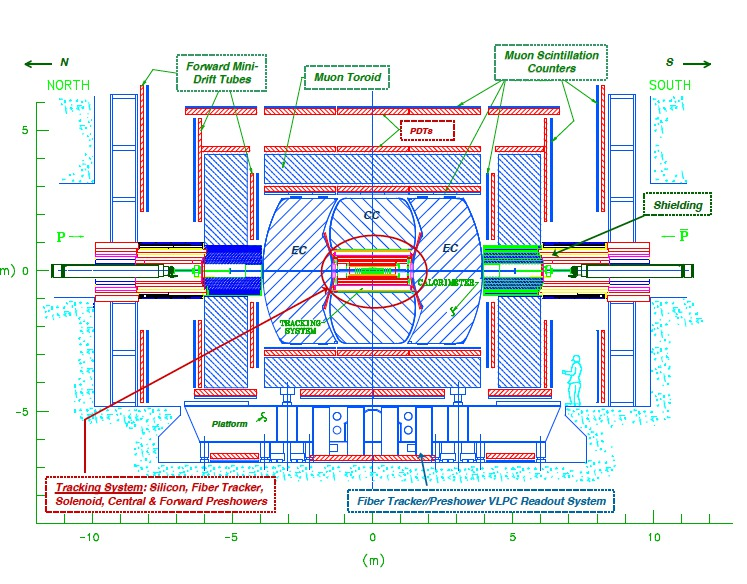
\includegraphics[width=0.95\linewidth]{./Images/02_D0_layout}%{00_upgraded_D0}
    %\caption*{upgraded D$\emptyset$ detector }
  \end{figure}
\end{frame}

